\documentclass{standalone}
\usepackage{tikz}
\usepackage{amsmath}

\begin{document}

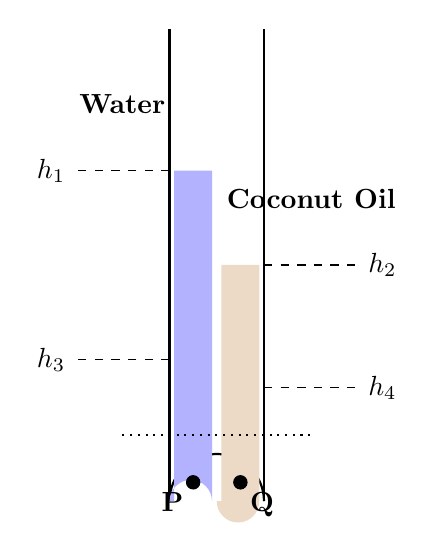
\begin{tikzpicture}[scale=1.2]
\draw[thick] (0,0) -- (0,5);
\draw[thick] (0,0) arc[start angle=180,end angle=0,radius=0.5cm];
\draw[thick] (1,0) -- (1,5);
\fill[blue!30] (0.05,0) -- (0.05,3.5) -- (0.45,3.5) -- (0.45,0) arc[start angle=0,end angle=180,radius=0.225cm];
\fill[brown!30] (0.55,0) -- (0.55,2.5) -- (0.95,2.5) -- (0.95,0) arc[start angle=0,end angle=-180,radius=0.225cm];
\draw[dashed] (0,3.5) -- (-1,3.5) node[left] {$h_1$};
\draw[dashed] (1,2.5) -- (2,2.5) node[right] {$h_2$};
\draw[dashed] (0,1.5) -- (-1,1.5) node[left] {$h_3$};
\draw[dashed] (1,1.2) -- (2,1.2) node[right] {$h_4$};
\draw[dotted, thick] (-0.5,0.7) -- (1.5,0.7);
\node at (-0.5,4.2) {\textbf{Water}};
\node at (1.5,3.2) {\textbf{Coconut Oil}};
\filldraw[black] (0.25,0.2) circle (2pt) node[below left] {\textbf{P}};
\filldraw[black] (0.75,0.2) circle (2pt) node[below right] {\textbf{Q}};
\end{tikzpicture}

\end{document}
